\section{Project: Icarus Overview}
\label{sec:overview}

Project: Icarus incorporates a novel airframe design paired with a highly
custom flight computer stack that blends together the hardware advantages of
fixed wing aircraft and multirotor aircraft in a hybrid-EVTOL aircraft with the
capability to transition  between multirotor and fixed wing flight. The
airframe is constructed using carbon  fibre and is designed to be lightweight
and durable.

Characteristics of the Project: Icarus airframe include a wingspan of 2.4 m and
a wing chord length of 0.4 m. The horizontal stabilizers has a span of 0.8 m,
chord length of 0.32 m, and the two vertical stabilizers, one attached at each
end of the horizontal stabilizer, are 0.3 m tall. The booms are 1.2 m long. The
NACA 64A210  airfoil was chosen for this aircraft.

\begin{figure}[ht]
        \centering
        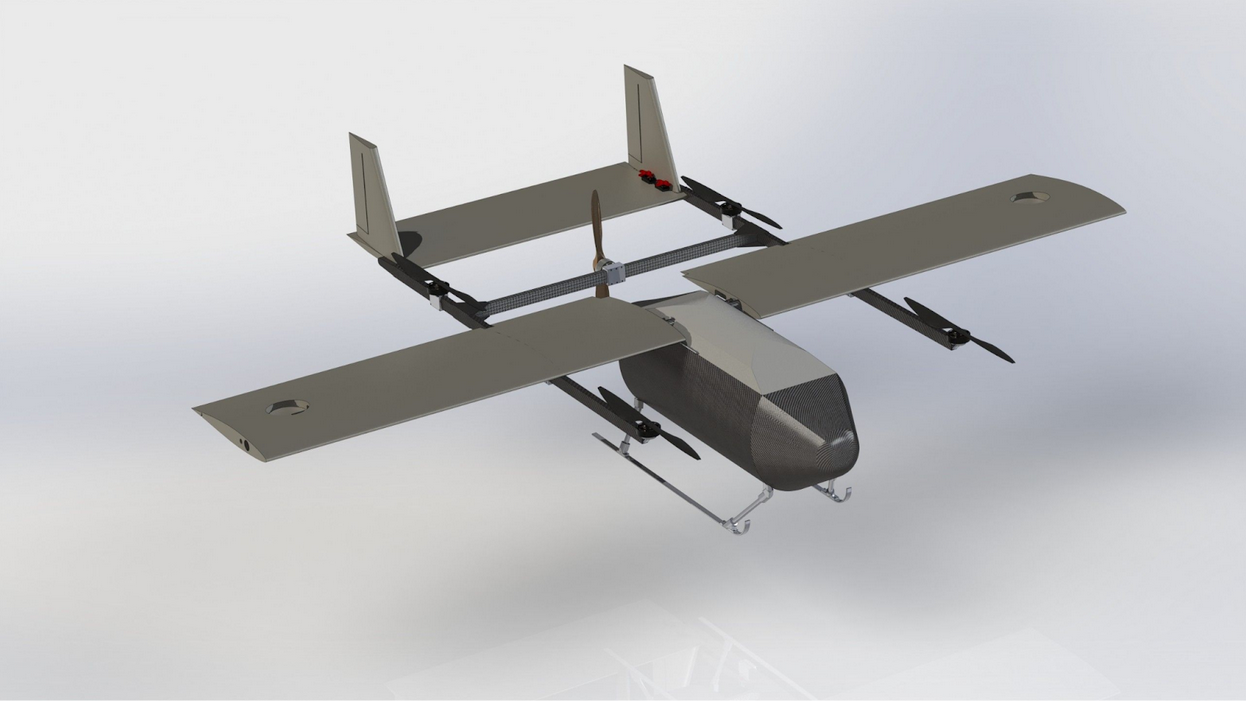
\includegraphics[scale=0.5]{frame}
        \caption{Project: Icarus airframe isometric projection}
\end{figure}

In terms of materials, the structural H-shaped frame of the aircraft, which
includes the two booms and the rear cross-beam, is made from 15 mm * 31 mm
rectangular carbon fibre twill tubing. The fuselage of the aircraft is made
from custom moulded carbon fibre sheets. The wing spar, (the carbon fibre tube
that runs through the wings, attaching to the H-frame at each boom), is 25 mm
diameter carbon fibre twill tubing. The wings and tail are made from CNC-cut
XPS foam. Paper and epoxy was used to coat the surfaces of these foam parts to
obtain a better surface finish and impact resistance. This, combined with the
carbon fibre construction, allows for a minimised weight footprint while
retaining good torsional rigidity and stiffness.

A number of assumptions with an added safety factor were considered to
determine that a surface area of at least $0.8 m^2$ would be necessary for the
aircraft to fly at 70 km/h. The aircraft as it exists now has a wing surface
area of $0.96 m^2$. The motor and prop combination that were chosen provide 8
kg of thrust, each, to facilitate a high thrust-to-weight ratio. The fuselage
was designed to be aerodynamic, with a focus on having laminar airflow being
directed towards the push motor. The aircraft is equipped with 6 seats using
four-point harnesses to secure passengers.

Internals of the fuselage will be discussed in the Passenger Safety section. As
an overview, the fuselage has a bay door on the port side, which sings open
downwards to form a staircase for passengers to board.

In order to meet the unique requirements for forward fixed wing flight as well
as vertical takeoff and landing, we to use VTOL specific locking motors that
are designed to run in short bursts. Paired with smaller propellers and higher
rotational velocity, this allows us to achieve similar amounts of thrust in a
lighter and more compact package. The push prop chosen was an APC 16*8x3
bullnose on a lower KV motor gives a 1:1 thrust ratio for a MTOW of 8 kg.
